\documentclass[titlepage,twocolumn,10pt]{article}
\usepackage[top=1in, bottom=1in, left=0.75in, right=0.75in, columnsep=20pt]{geometry}
%\usepackage[framed,numbered,autolinebreaks,useliterate]{mcode}
\usepackage{amsmath,textcomp,amssymb,geometry,graphicx,enumerate,listings,graphicx,multirow}
\newenvironment{qparts}{\begin{enumerate}[{(}a{)}]}{\end{enumerate}}

\usepackage{ebgaramond}
%\usepackage[T1]{fontenc} % Use 8-bit encoding that has 256 glyphs
%\linespread{1.05} % Line spacing - Palatino needs more space between lines
%\usepackage{microtype} % Slightly tweak font spacing for aesthetics

%\usepackage[hmarginratio=1:1,top=32mm,columnsep=20pt]{geometry} % Document margins
%\usepackage{multicol} % Used for the two-column layout of the document
%\usepackage[hang, small,labelfont=bf,up,textfont=it,up]{caption} % Custom captions under/above floats in tables or figures
\usepackage{booktabs} % Horizontal rules in tables
\usepackage{float} % Required for tables and figures in the multi-column environment - they need to be placed in specific locations with the [H] (e.g. \begin{table}[H])
\usepackage{hyperref} % For hyperlinks in the PDF

%\usepackage{paralist} % Used for the compactitem environment which makes bullet points with less space between them

\usepackage{titlesec} % Allows customization of titles

\usepackage{fancyhdr} % Headers and footers
\pagestyle{fancy} % All pages have headers and footers
\fancyhead{} % Blank out the default header
\fancyfoot{} % Blank out the default footer
\fancyhead[C]{2015 RASC-AL Robo-Ops Competition \hfill \today} % Custom header text
\fancyfoot[RO,LE]{\thepage} % Custom footer text

%----------------------------------------------------------------------------------------
%	TITLE SECTION
%----------------------------------------------------------------------------------------
\title{\vspace{-15mm}\fontsize{24pt}{10pt}\selectfont\textbf{CAL-Rover Project Plan Proposal}} % Article title

\author{
    \large University of California, Berkeley \\ % Your institution
    [5mm]
    \normalsize \textsc{Team Leads: Piyush Prakash, Brian Lau, Sirisha Varigonda, Casey Getz,}\\[0mm]
    \normalsize \textsc{Terence Cho, Akhil Devarakonda, Wesley Guo, Tony Yau}\\[3mm]
    \normalsize \textsc{Team Members: Aaron Feldman, Bahador Behdad, Jeremy Cook, Rohan Deshpande}\\[0mm]
    \normalsize \textsc{Howard Nguyen, Eric Nguyen, Nikhil Sathe, Ryan Goy, Sean Luna, Kevin Fan}\\[0mm]
    \normalsize \textsc{Harrison Agrusa, Theodore Teo, Rachel Zhang, Davina Boedijono, Henry Lei}\\[0mm]
    \normalsize \textsc{Risa Pesavento, Thomas Kim, John Smail, Yu-Chieh Lee}\\[3mm]
    \normalsize \textsc{Faculty Advisor: David M. Auslander}\\[6mm]
    \includegraphics*[width = \textwidth]{images/robot.png}
}

%\titlehead{\centering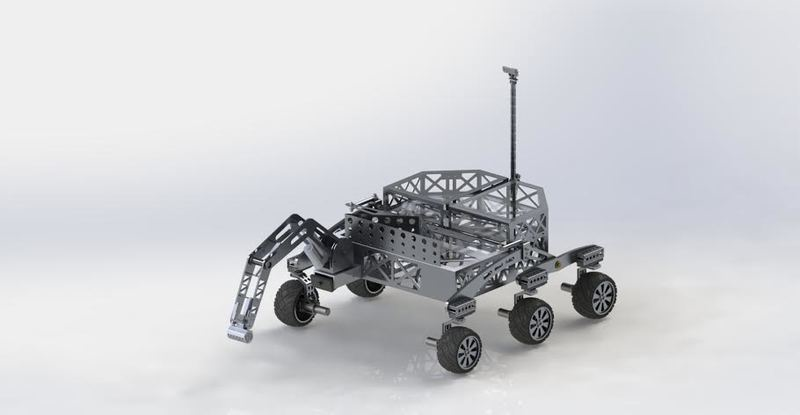
\includegraphics[width=6cm]{robot.png}}
%----------------------------------------------------------------------------------------

\begin{document}

\maketitle % Insert title

\thispagestyle{fancy} % All pages have headers and footers

%----------------------------------------------------------------------------------------
%	ABSTRACT
%----------------------------------------------------------------------------------------

%\begin{abstract}

%\noindent \lipsum[1] % Dummy abstract text

%\end{abstract}

%----------------------------------------------------------------------------------------
%	ARTICLE CONTENTS
%----------------------------------------------------------------------------------------

%\begin{multicols}{2} % Two-column layout throughout the main article text

    \section{Introduction}
    CAL-Rover is the University of California - Berkeley's entry into NASA's 2015 RASC-AL Robo-Ops competition. Upon completion, its instrument suite will feature three cameras (one of which will have pan and tilt capability) and a 5-DOF manipulator arm. In its stowed configuration, the rover fits within an 94.4 cm by 87.2 cm by 46.4 cm box, which fits within the maximum envelope of 1m x 1m x 0.5m. It is expected to have a total mass of 39.69 kg, which is well below the competition's maximum limit of 45 kg.

    The mission goal for CAL-Rover is to traverse the Johnson Space Center (henceforth referred to as JSC) Rock Yard and acquire as many colored rock samples as possible within a one-hour time frame. This document will explain the systems implemented on CAL-Rover, how they have been improved from previous designs, and why it should be considered for the 2015 competition season. All physical dimensions are given in MKS units, but since most domestic part and material suppliers list their products in imperial units, these dimensions will be displayed in parentheses where appropriate.
    \section{Systems}
    CAL-Rover's current design benefits greatly from previous competition experience. Through analysis and testing of the shortcomings of our previous designs, CAL-Rover is UC Berkeley's best design yet. The 2015 design focuses on increased mobility and dexterity of the rover.

    To accomplish these goals, we completely redesigned the chassis, drivetrain, and suspension systems from previous designs. We made these drastic improvements to allow for weight reduction, better mobility, and more precise positioning. The final goal is to have a more robust rover that can be ensured to work as designed.

    \subsection{Chassis}
    The chassis consists of eight structural plates that create the enclosure. Each plate will be water jetted from 100 thou thick 6061-T6 Aluminum sheets. To reduce weight, structural sheets incorporate truss designs with rectangular and triangular extruded cuts. Structural plates will be TIG welded, then wrapped in clear MonoKote to seal the inside from the environment. A thin bar outlines the top of the chassis to maintain structural integrity of the frame. A gap is left between the left half and the right half of the rear of the chassis to accommodate placement of the camera mast.

    In order to access the internal structure of the rover, two hinged doors in the back-left and back-right corners open downward and are secured at the top with quick release pins. The top of the rover will also be used to access the internal components. The top roof will be split into two halves, each supported by the top bar and wrapped in clear MonoKote allowing direct visibility to internal components.

    One of the improvements from last year's chassis design is space efficiency. This year's design utilizes stacking of the electrical components in a more compact frame. In order to attain this, a shelf supported by bolts is placed inside the chassis to efficiently allocate vertical space. The shelf itself will consist of two parts: a 100 thou thick 6061-T6 Aluminum sheet with triangular truss designs to reduce weight and a 75 thou polycarbonate sheet upon which electrical components will be placed.

    The front plate of the chassis will house the mounting for the manipulator arm, while the lower  roof will support the rock box and differential bar. The rock box itself will consist of three plates of sheet metal welded together at the edges into a triangular design. The main bottom frame of the chassis will have a similar setup to the shelf; it will consist of a water jetted aluminum sheet and a sheet of ABS PC Plastic placed directly on top to support internal components.

    \begin{figure}[H]
        \centering
        \includegraphics*[width = 7cm]{images/chassis.png}
        \caption{Chassis}
    \end{figure}

    \begin{figure}[H]
        \centering
        \includegraphics*[width = 6cm]{images/chassistop.png}
        \caption{Top view of chassis}
    \end{figure}

    \subsection{Suspension}
    In previous years, Berkeley's rovers have had simple rocker suspension systems. This year, CAL-Rover features a rocker-bogie suspension system with a bar differential. The overall suspension characteristics are similar to previous but with two extra wheels for increased rover stability. The differential constrains the motion of the two arms relative to each other. When one arm tilts upward a certain angle, the other arm tilts in the opposite direction by an equivalent angle. The movement of the rocker-bogies maintains at least four wheels in contact with the ground at any point in time. As the rover drives over obstales, the chassis remains relatively horizontal, making the JSC Rock Yard easier to traverse.

    With the rocker-bogie in the neutral position (all six wheels on flat ground), the main body of the rover sits at 20cm above the ground. In the event that it runs over a rock or other obstacle, the rover is able to climb over obstacles 10cm in height through the rotation of the rocker-bogie system.

    \begin{figure}[H]
        \centering
        \includegraphics*[width = 7cm]{images/suspover.png}
        \caption{The suspension system in isolation}
    \end{figure}

    \begin{figure}[H]
        \centering
        \includegraphics*[width = 7cm]{images/suspdisp.png}
        \caption{Image showing the capability of the wheels to vertically displace 13cm, which demonstrates its ability to overcome 10cm obstacles.}
    \end{figure}

    \subsection{Swerve Drive}
    \begin{figure}[H]
        \centering
        \includegraphics*[width = 6cm]{images/swerve.jpg}
        \caption{Swerve module}
    \end{figure}

    \begin{figure}[H]
        \centering
        \includegraphics*[width = 9cm]{images/swerveexp.jpg}
        \caption{Swerve module exploded view}
    \end{figure}
    The swerve drive design has been completely revamped from last year. Motivations for this change include the desire to minimize weight and bulkiness of each module as well as to reduce manufacturing times. CAL-Rover boasts six swerve modules, each of which are individually operable (shown in Figure 3). The swerve module leg is the heart of the new design.. The leg distributes the weight of the rover evenly to the hub of the wheels through a double bearing assembly. Through this design,the drive motors are spared the weight of the rover.

    Module heading is controlled by a SPG785-CM Servo with a 7:1 ratio gearbox. Each servo can provide 9.05 N-m of torque, which is more than sufficient to turn the modules. Propelling the 15.24 cm diameter wheels are Banebot PDX104 motors with 104:1 ratio gearboxes. To navigate the rock yard, the max torque required is around 20 N-m. This result was calculated assuming a worst case scenario of all the weight on one wheel. Assuming the competition limit weight of 45 kg and a coefficient of friction $\mu = 0.6$, the normal force and friction force on the wheel are 441 N and 265 N respectively. The motor torque required to turn the wheels in this scenario is the friction force times the radius of the wheel (0.0762 m), which turns out to be around 20 N-m. Each PDX104 motor can individually supply a stall torque of 67.23 N-m, which is plenty to drive the rover, even on inclines.

    The major parts of the swerve modules include the leg and wheel hub, which are both made from 6061-T6 aluminum. To validate the strength of these parts, FEA was conducted using Solidworks Simulation. The results of these calculations can be seen in Figure 4. The worst case scenario was assumed to be the competition weight limit of 45 kg being stranded on one wheel, which provided a force of 441 N on the wheel. The max deformation for both parts was less than 1 mm (the deformations in the pictures are greatly exaggerated for visual purposes).

    \begin{figure}[H]
        \centering
        \includegraphics*[width = 7cm]{images/fealeg.jpg}
        \caption{Swerve module}
    \end{figure}

    \begin{figure}[H]
        \centering
        \includegraphics*[width = 7cm]{images/feawheel.png}
        \caption{Swerve module exploded view}
    \end{figure}

    Last year, the wheels were designed as machined steel and aluminum pipe caps. However, the machining process left the aluminum pipe caps too deformed to use properly, so this year we are going to weld aluminum round tube and sheet to create the wheels. This design will be  machinable with constant quality.  Last year we used a 3-layer Styrene Butadiene Rubber treading, but that proved to be less resistant to wear than we would have liked. Therefore, this year the tires will be made in house, using a two-part polyurethane mix that has a shore hardness of 70A, which is comparable to car tires.

    \subsection{Manipulator}
    CAL-Rover's manipulator arm benefits from five degrees-of-freedom: three linearly-actuated hinges along the arm, a rotational base plate for yaw movement, and a linearly-actuated end effector to manipulate the claw. A five degree-of-freedom design increases the positional precision of the end effector and allows it to operate along various distances and directions from the rover. As a result, the arm's maneuverability and efficiency increases compared to the previous 3-DOF arm that could only gather rocks within a fixed distance from the rover. The arm is maneuvered primarily by a set of Firgelli linear actuators. The angled first boom is driven by a Figerlli FA-PO-150-12-2 actuator with a 50.8 mm (2 in) stroke and maximum load of 667 N (150 lbs). The second straight boom is supported by a Firgelli L16 series actuator with a 50 mm stroke and maximum load of 100N. Finally, both the wrist joint and end effector are driven by Firgelli L12 series actuators with 30 mm and 10 mm strokes respectively.
     
    \begin{figure}[H]
        \centering
        \includegraphics*[width = 8cm]{images/manip.png}
        \caption{Overall view of the manipulator, showing the two booms, main linear actuator and end effector}
    \end{figure}

    Linear actuators were chosen over right angled motors for two main reasons. First, with a 46N back drive force on the L16 models and 100N back drive force on the L12 models, we can maintain force without power usage. Second, the ease of use and built-in positional feedback allows greater precision control over the arm. Although linear actuators do individually have a reduced range of motion compared to traditional DC or servo motors, proper placement of actuators and selection of stroke lengths ensures that the overall range of motion of the arm is more maneuverable than previous years' designs. The high maximum loads were chosen to ensure that the actuators can drive the arm even throughout the full range of loading conditions.
    
    The only traditional DC motor on the arm is the Pololu 9.7:1 metal gearmotor in the arm's base housing used for rotation. A 90:1 worm drive gear ratio was chosen to both minimize the torque required from the motor and to allow for very precise yaw adjustments. A worm drive also protects the motor itself by ensuring that the unexpected forces on the arm cannot backdrive the motor shaft. This motor can output up to 10.8 N-m of torque, which is comfortably larger than the 0.13 N-m of torque required to turn the arm at the given gear ratio. 
    
    The arm can sweep a full 360 degrees, and pick up samples within an arced region of 10.16 cm and 40.64 cm from the edge of the arm base. This large range of motion eliminates the need to reposition the rover to collect samples.

    \begin{figure}[H]
        \centering
        \includegraphics*[width = 8cm]{images/manipdim.png}
        \caption{Diagram showing horizontal range of the arm ($dX$). The orange line is the ground level}
    \end{figure}

    The end joint ``wrist" is driven with a rack and pinion style drive. A gear rack mounted to the linear actuator gives the wrist 171° of rotational motion. The end effector is directly mounted to the wrist shaft with one fixed claw and the other free to rotational motion. Using a 10 mm stroke L12 actuator in conjunction with a rack and pinion, the end effector is allowed up to 114° of opening rotation. Sample collection is achieved through two curved shovels that interlock around samples up to 8 cm in width. Back drive force of the linear actuators ensures that the claw can remain clamped down around large samples without power.
    
    \begin{figure}[H]
        \centering
        \includegraphics*[width = 8cm]{images/endeff.png}
        \caption{Close up of rack, pinion, and end effector. 10 mm stroke actuator on the left, 30 mm stroke actuator on right}
    \end{figure}

    \subsection{Command and Control}
    Cal-Rover will be commanded via an internet connection with the home computer back in UC Berkeley. There are two main computers in this setup: a command computer back at home base, and a control computer which is onboard the rover. On the command computer, a GUI written in Python handles inputs given by an Xbox 360 controller and a Logitech joystick that map the inputs to commands that are transmitted to the rover via a TCP socket, also established by Python scripts running on both the command computer and the control computer. The control computer will be a Acer Chromebook, which was selected for its small form factor and ease of debugging. The Chromebook will be running the Ubuntu Linux distribution.  The Chromebook interprets the commands and routes them to the appropriate systems for actuation. Two Arduino MEGAs drive actuation of all mechanical systems onboard the rover, with one dedicated for the swerve drive and another dedicated to the arm and any other actuators for the cameras. Each time the Arduino successfully executes a command, verification is sent back to the ultrabook and subsequently back to the control computer.

    The work of controlling the rover will be split into two main teams. One team will handle driving the rover, and one team will handle controlling the manipulator arm. This is because we believe both systems are quite mechanically complex and require many input modes. Since we do not expect to drive and acquire samples at the same time, these teams will rotate, with the driving being controlled with the Xbox controller and the arm actuation being controlled by the Logitech joystick. Both teams will be able to change and update their sensitivity settings through the GUI as well as see the state of their systems, e.g. the orientation of their systems at all time without the need for a camera feed. For the arm system, this will be achieved by utilizing the internal feedback of the linear actuators used to control the arm. With this feedback, we will be able to calculate the position of the arms at all times. For the swerve drives and orientation of the wheels, we will rely on encoders placed directly on top of the motors. Visual feedback will be provided by multiple camera streams, and different feeds can be accessed by the GUI. For ease of control while picking up rocks, a camera connected to the arm will provide a view that will ease the job of the person controlling the arm. Because of this camera there will be no worry about calculating the depth of the rocks from the front base camera. A GPS location of the rover will also be visible on the GUI, overlayed over a map of the the competition area. These new features from last year will greatly increase the precision of control for the systems controller back at home base.

    \begin{figure}[H]
        \centering
        \includegraphics*[width = 9cm]{images/gui.png}
        \caption{A mockup of the proposed GUI}
    \end{figure}

    \subsection{Communications and Audio-Video Streaming}
    The onboard Acer Chromebook will act as the center of communications for the rover.  The Chromebook will be connected via WiFi to a Verizon MiFi LTE modem.  This 4G connection will serve as the link between the robot and the home base.  The amount of bandwidth provided should be enough to reliably send control commands and stream audio and video.  Last year, we found that cellular modems generally do not allow port forwarding over the internet, resulting in difficulty running server-like services on the robot.  To combat this and allow for more data security, we will connect the rover computer to a virtual private network, which will allow us to use ports on local IP addresses.  This year, we will also attach a USB GPS receiver to the Chromebook.  The coordinates provided by the receiver will be sent over a TCP socket to the control computer, and will be used to display the rover's location, as was described in the previous section.  Additionally, we will be using a new serial message protocol for communicating between the Chromebook and the microcontrollers.  The new message protocol will enhance our ability to perform error detection xon the Arduinos and ensure that the correct motor control messages are received.

    The central computer will be connected to three USB cameras.  These cameras will provide the operator with a good view of the rover and all of its surroundings.  One of these cameras will also record audio.  The video and audio will be streamed between the onboard computer and the control station through the use of a RTP streaming server that runs on the robot.  This will be written in Python using the GStreamer API.  GStreamer can handle the full gamut of multimedia streaming needs, from reading frames from the webcam to compressing the video using the H264 protocol to starting an RTP webserver to transmit the video over the internet.  The use of GStreamer will allow us to use more efficient video codecs than the Motion JPEG based solution from last year.  This will allow us to stream higher resolution video at higher frame rates.  Additionally, instead of relying on a simple HTTP server for supplying the video file, we will utilize the Real-time Transport Protocol, which is built specifically for efficient multimedia transmission.  The remote control side will also use the GStreamer library to receive, decompress, and show the data in a GUI window.  To compensate for potential bandwidth issues with the cellular network, we will allow the camera streams to be switched on and off remotely during the competition.
    \subsection{Power}
    In order to power Cal-Rover, we will use a similar power distribution system to last year, with a set of batteries delegated to the drivetrain and arm motors and an isolated battery for powering the computing and communication equipment.  However, given that our drivetrain now includes six motors our current draw over one hour will be somewhat higher, approximately 32Ah.  Thus, we will use an array of five Zippy FlightMax 8000mAh LiPO batteries in parallel to power these high-draw motors.  As each battery can supply a continuous current of 240A at 14.8V, we can support a continuous current draw of 1200A, if need be.   This is more than sufficient to supply power to the drive motors under nominal load and maintain power in stall conditions for short periods of time.  The central computer, microcontroller boards and cellular modem are powered by an additional isolated 8000mAh battery.  This ensures that power is provided consistently to the onboard electronics.  Also, both the cellular modem and the central computer have integrated batteries that can power the device if power from the external battery is cut.

    In order to regulate voltages delivered to the hardware, we have fabricated DC-DC converter circuit boards.  These boards provide consistent 12V, 6V, and 5V rails to power the complete range of onboard devices and motors.  The regulator boards also have high-power diodes that prevent backflow of current into the batteries.  The 12V rail is connected to ground via a filter capacitor.

    \subsection{Cameras}
    Attached to the rear of rover chassis is a camera mast which sustains the main directional camera. The mast stores flat across the top of the chassis and extends to a maximum height of 15 inches above the chassis through a geared pulley system. Utilizing a Pololu 100:1 Micro Metal Gearmotor in conjunction with a 20:1 worm gear set and 2.4:1 cable reel gear ratio, the pulley system can provide a maximum of 8.47 N-m of torque to lift the camera mast. At the worst case scenario, the mast will require 0.53 N∙m of torque to lift the mast to full upright.

    The main directional camera sits at the end of the camera mast. It is attached to two micro continuous-rotation servos providing 360° panning of the terrain and 180° range of tilt adjustment.
    An additional camera will be attached to the arm in order to give the rover operators increased control over the manipulator by providing a view of the ground. This camera will be attached to the second boom and remain pointed out along the length of the boom

    \section{Timeline}
    The proposed build and test schedule for Cal Rover is described on the next page in Table 1. Most action items are split into two or three phases. For mechanical components, there will usually be a machining phase and an assembly phase. For the electromechanical components, items are interfaced with the Arduino and the control software is then configured to interface with the hardware. We have also allotted a month of buffer time in which to debug, test and catch up on slipped production days.

    \begin{table*}[P]
        \begin{tabular*}{\textwidth}{l  l  l}
            \textbf{Timeframe} & \textbf{Action Item} & \textbf{Description} \\
            \hline \hline
            27 Oct - 3 Nov & Purchase Raw Materials & 27 Oct - 3 Nov: Purchase materials for mechanical systems \\
            & & 27 Oct - 3 Nov: Purchase communications and electrical hardware\\
            \hline
            3 Nov - 5 Dec & Building Arm & 3 Nov - 25 Nov: Machining arm parts\\
            & & 26 Nov - 5 Dec: Assembling arm\\
            \hline
            3 Nov - 28 Feb & Building Suspension & 3 Nov -  5 Jan: Machine parts\\
            & & 5 Jan - 31 Jan Assemble Parts\\
            \hline
            3 Nov- 5 Dec & Building Swerve Modules & 3 Nov - 14 Nov: Waterjet and machine swerve support arm \\
            & & 15 Nov - 30 Nov: Manufacture other swerve parts\\
            & & 1 Dec - 5 Dec: Assembly of swerve modules\\
            \hline
            5 Jan - 18 Mar & Building Chassis & 5  Jan - 28 Feb: Cutting/drilling chassis frame components \\
            & & 1 Mar - 18 Mar: Send chassis out for welding \\
            \hline
            10 Mar - 18 Mar & Camera Integration &  10 Mar - 18 Mar: Build camera masts \\
            \hline
            18 Mar - 1 Apr & Complete Mechanical Systems Integration & 18 Mar - 21 Mar: Mount arm to chassis \\
            & & 18 Mar - 21 Mar: Mount swerve\\
            & & 18 Mar - 21 Mar: Mount cameras\\
            & & 13 Mar - 1 Apr: Integrate electronics\\
            \hline
            31 Mar - 15 Apr & Complete Software Systems Integration & 31 Mar - 15 Apr: Finalize GUI design \\
            & & 31 Mar - 15 Apr: Program Arduino to interface with arm\\
            & & 31 Mar - 15 Apr: Program Arduino to interface with swerve drive\\
            \hline
            31 Mar - 30 Apr & Communications Setup & 31 Mar - 13 Apr: Tune video transmission \\
            & & 31 Mar - 31 Apr: Clean up video display/GUI \\
            \hline
            21 Apr - 3 Jun & Testing/Debugging & Apr 1 - 16 May: Test and debug all systems \\
            & & 16 May - 3 Jun: Run full simulated tests of debugged rover\\
            \hline
            30 Mar & Rover Assembly Completed &  \\
        \end{tabular*}
        \caption{The build and test schedule for the rover}
    \end{table*}
    
    \section{Public Engagement}
    Cal Rover already has a website hosted by the Open Computing Facility at Berkeley. Currently, it will be updated over the course of next semester. It can be accessed at http://aiaa.berkeley.edu. To additionally engage the public about this project, however, we will also continue the team facebook which will log progress made on the rover.

    Once physical rover development begins, we also have plans to participate in outreach programs with other clubs on campus. In the Spring, an E4K (Engineering for Kids)  occurs where we will show off our rover to help spread STEM interest amongst children. Additionally, we will collaborate with the Engineering Student Council in Engineering week, which is an event meant to showcase engineering to the general publics in UC Berkeley.

    UC Berkeley also has a school open-house called CAL-day in which student groups are encouraged to showcase their organizations and projects they are working on. We participated in CAL-Day last year and hope to do so again this year to hopefully encourage the incoming freshmen to pursue STEM careers while they are in college.

    Finally, for the livestream, we will be streaming a composite of the different rover camera views and sound from an onboard microphone.  We will be using either UStream or Google Hangouts on Air to stream the multimedia feeds to the masses.  These services will allow anyone with access to the internet to watch our rover's progress during the competition.

    \section{Team Skills and Facilities}
    The Cal-Rover team is fortunate to be composed of and led by highly competent individuals. For the 2014-2015 competition, all leads have been team members during at least one previous Robo-Ops competition, providing them a full range of useful competition knowledge and experience.  The team members are listed in Table 2. 

    \begin{table*}[P]
        \begin{tabular*}{\textwidth}{l  l  l}
            \textbf{Name} & \textbf{Role} & \textbf{Relevant Experience/Skills} \\
            \hline \hline
            David Auslander, PhD & Advisor & - Professor of mechatronics/controls \\
            & & - Has worked on many projects at Space Sciences Laboratory at Berkeley \\
            \hline
            Piyush Prakash & Team Lead & - Previous Chassis/Suspension Lead (2013-2014) \\
            & & - Design Lead at UC Berkeley FSAE \\
            & & - Proficient in SolidWork and AutoCAD \\
            & & - Machine shop trained \\
            \hline
            Brian Lau & Team Lead & - Previous Chassis/Suspension Lead (2013-2014) \\
            & & - Design Lead at UC Berkeley FSAE \\
            & & - Proficient in SolidWork and AutoCAD \\
            & & - Machine shop trained \\
            \hline
            Casey Getz & Communications Lead & - Previous Communications Lead (2013-2014) \\
            & & - Proficient in C/C++, Python, Network Programming\\
            & & - Worked as intern at Amazon Lab 126 \\
            \hline
            Akhil Devarakonda & Drivetrain Lead & - Previous Chassis/Suspension member (2013-2014) \\
            & & - Machine shop trained \\
            \hline
            Sirisha Varigonda & Chassis/Suspension Lead & - Previous Manipulator member (2013-2014) \\
            & & - Machine shop trained \\
            \hline
            Wesley Guo & Manipulator Lead & - Previous Manipulator member (2013-2014) \\
            & & - Machine shop trained \\
            \hline
            Terence Cho & Controls Lead & - Previous Drivetrain/Controls member (2013-2014) \\
            & & - Machine shop trained \\
            \hline
            Tony Yau & Electrical Lead & - Previous electrical member (2013-2014) \\
        \end{tabular*}
        \caption{The administrative team roster for 2014-2015}
    \end{table*}

    The Cal-Rover team will have access to three major facilities to complete the construction of the rover. For machining the various parts needed, we have access to the Etcheverry student machine shop, which is equipped with milling machines, lathes, bandsaws, and drill presses, which many of our team members are or will be trained to use for the spring semester. For the electrical components, we have access to the SuperNode hackerspace in Berkeley, which is equipped with bench-top oscilloscopes, power supplies and soldering irons. Assembly of the rover is most likely to occur either in the Etcheverry machine shop or in room 120AB in Bechtel hall, which is the third facility available to us.
   
    \begin{figure}[H]
        \centering
        \includegraphics*[width = 4cm]{images/etch.jpg}
        \includegraphics*[width = 4cm]{images/cory.jpg}
        \includegraphics*[width = 5cm]{images/becht.jpg}
        \caption{Etcheverry machine shop, Cory Hall, and 120AB Bechtel, respectively} 
    \end{figure}

    \section{Lesson Learned}
    This report is UC Berkeley's third entry into the competition and with our experience, we have made some important changes to the design and design process. While in the past, we attempted to use all the space provided for the rover, this year we decided to look at spatial efficiency over total use. This has allowed us to significantly decrease the size of our chassis. Additionally, from our performance in the previous year's competition, we have designed our mechanical system with the electronics in mind; for example, the polycarbonate plates were added to the chassis to insulate the electronics from the chassis. Also at the previous year's competition, we learned that our rover's bulkiness was a large weakness when it came to performance. For example, the swerve drive's bulk impeded its ability to rotate and the rover's width created issues when turning the wheels through tank drive. This year we fixed those issues by completely redesigning the swerve drive and reducing the width of the chassis.
  
    \section{Statement of Preparedness and Conclusion}
    The Cal-Rover team believes that we are sufficiently prepared to enter and compete in the 2015 Robo-Ops competition. All of the critical systems have been fully designed, and technical drawings and bills of materials have been drafted for each subsystem. Additionally, we have competed in the competition before, and have proven ourselves to be able to build a rover within the time constraints. We have had time to critically look at our past years of design and have created a new design to improve upon the previous year's flaws. 

    Additional factors that will have to be closely monitored are the build schedule and regular updating of the team website and Facebook page. To limit the chance that bottlenecks will stall rover development, the proposed timeline allows for some buffering in case some components fall behind schedule. That being said, however, team leads will ensure that manufacturing remains on track as much as possible.

\end{document}
